
\begin{figure}[h!]
    \centering
    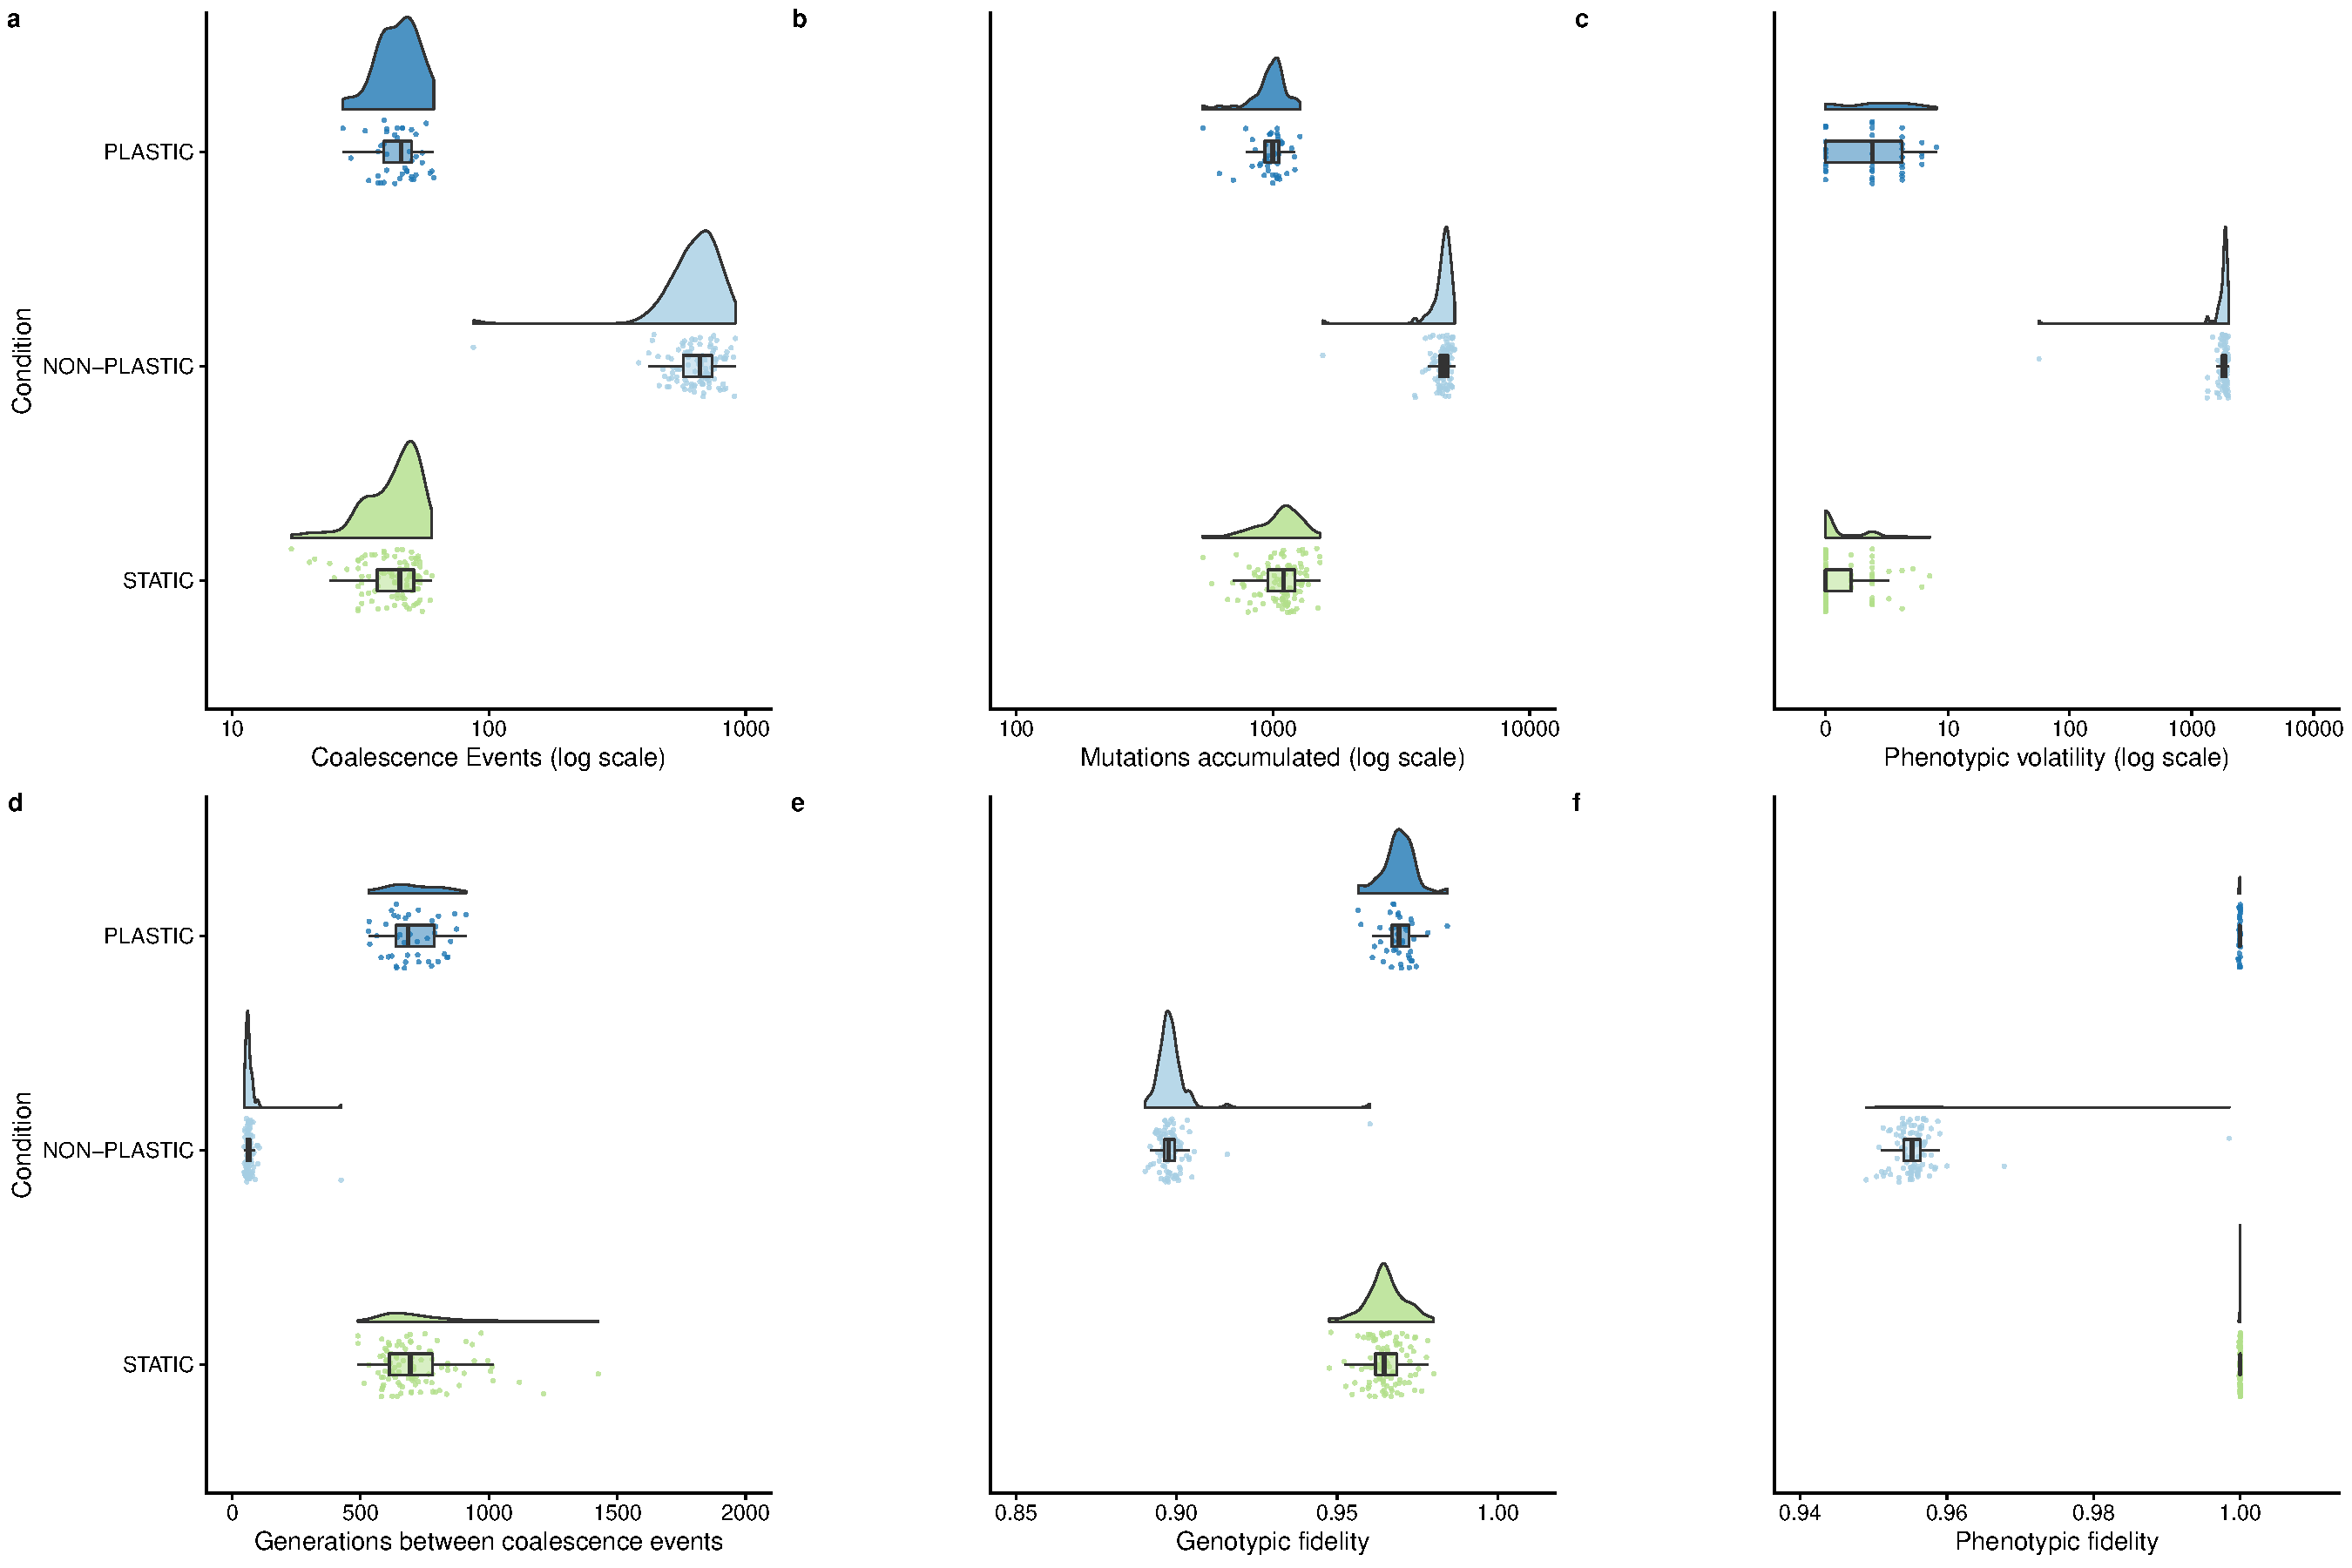
\includegraphics[width=1\textwidth]{media/evolutionary-change-full-panel.pdf}
    \caption{\small
    \textbf{Evolutionary change.}
    Raincloud plots \citep{allen_raincloud_2019} of 
    (a) coalescence event count, 
    (b) mutation count, 
    (c) phenotypic volatility, 
    (d) average number of generations between coalescence events,
    (e) genotypic volatility,
    and (f) phenotypic volatility.
    See Table \ref{tab:metrics-definitions} for descriptions of each metric.
    The top row of plots describe the magnitude of evolutionary change observed for PLASTIC, NON-PLASTIC, and STATIC populations.
    The bottom row of plots describe the rates of evolutionary change for each treatment.
    Each plot is annotated with statistically significant comparisons (Bonferroni-corrected pairwise Wilcoxon rank-sum tests).
    % test statistics given in supplement.
    % For each metric, we found that the NON-PLASTIC treatment exhibited both a larger magnitude and a higher frequency of evolutionary change during our experiment. 
    Note that adaptive phenotypic plasticity evolved in \evolutionaryChangeRatePlasticReps\ of \evolutionaryChangeRateReplicates\ replicates from the PLASTIC treatment during phase one of this experiment; we used this more limited group to found the \evolutionaryChangeRatePlasticReps\ phase-two PLASTIC replicates from which we report these PLASTIC data.
    }
    \label{fig:evolutionary-dynamics}
\end{figure}